\input{taskinfo.tex}
\taskheader

\newcommand{\TranslationPageOf}[2]{Page #1 of #2}
\newcommand{\TranslationDate}{April 8 -- April 12, 2013}
\newcommand{\TranslationDay}{Day 0}
\newcommand{\TranslationTL}{Time limit:}
\newcommand{\TranslationML}{Memory limit:}
\newcommand{\TranslationTLUnit}{sec per test case}
\newcommand{\TranslationMLUnit}{MB per test case}
\newcommand{\TranslationSampleSingular}{Example}
\newcommand{\TranslationSamplePlural}{Examples}
\newcommand{\TranslationSampleInput}{Input}
\newcommand{\TranslationSampleOutput}{Output}
\newcommand{\TranslationLimits}{Limits}

\newcommand{\TranslationTaskName}{Cheer the Worm Up}

\newcommand{\countrycode}{ENG}

\begin{document}
\heading{Cheer the Worm Up}

Willy Worm has suffered from a lack of attention since everyone is communicating via Facebook only -- no-one is talking to worms any longer! His owner wants to cheer him up, so he surprises him by putting some of Willy's favourite stones in his cave. Unfortunately, the stones are quite big and Willy wants to know how long he may grow so that he still fits in his cave. Help him.

Willy's cave is a grid of $5\times 5$ fields, some of which are occupied by stones. Each field can be denoted by a pair of coordinates $(x, y)$ with (1, 1) in the upper left corner.

When grown to length $n$ he needs to fit in his cave a sequence of fields $a_1,\dots,a_n$ with the following properties:

\begin{itemize}
\item Willy's favourite position is the lower left field of his cave, so he puts his head there: \\ $a_1 = (1, 5)$.
\item Fields $a_i$ and $a_{i + 1}$ have one border in common for all $i=1,\dots,n-1$.
\item $a_i \neq a_j$ for all $i\neq j$, which means that Willy does not intersect himself.
\item Of course no field $a_i$ is occupied by a stone.
\end{itemize}

\begin{figure}[h!]
\begin{center}
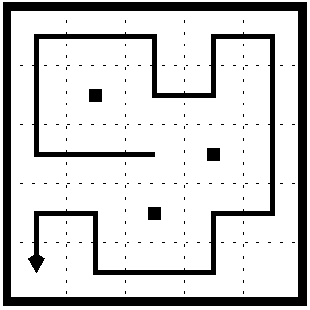
\includegraphics[width=1.29in]{fig1}
\end{center}
\caption{Willi and three stones in the cave.}\label{fig1}
\end{figure}

Write a program that calculates for a given number of stones and their positions the maximum length Willy may grow to, so that he still fits in his cave.

\subsection*{Input}

The first line contains the number of stones $M$ ($0 \le M \le 24$). The following $M$ lines contain pairs of coordinates $x$ $y$ ($1\le x, y\le 5$), giving the positions of the stones. You can assume that the lower left field (1, 5) is always empty and no two stones are placed on the same field.

\subsection*{Output}

The only line to be written contains the maximum length Willy may grow to, so that he still fits in his cave.

\subsection*{Constraints}
\constraint1

In testcases worth 40 points: \constraint2

\subsection*{Sample}
\showcases

\subsection*{Limits}
Time Limit: \timelimit \\
Memory Limit: \memlimit

\end{document}
